\nonstopmode
\documentclass{beamer}

\mode<presentation>
{
\usetheme{sts}

\setbeamercovered{transparent}
}

%\documentclass[handout]{beamer}
%\includeonlylecture{week12}

\usepackage{pdfpages}
\usepackage[utf8]{inputenc}
\usepackage[T1]{fontenc}
\usepackage{import}
\usepackage{times}
%\usepackage{pgf}
\usepackage{ctable}

\usepackage{listings}%[2000/08/23]
\usepackage{lstlangampl} % syntax file, I added some more keywords like 'display'

%\usepackage{graphicx}
%\usepackage{multicol}

%\usepackage{tikz}

\newcommand{\UMLType}[1]{\textbf{#1}}
\newcommand{\UMLReference}[1]{\emph{#1}}
\newcommand{\ATGType}[1]{\textsl{#1}}

\lstnewenvironment{java}
    {\lstset{language=java,basicstyle=\scriptsize,frame=}}
    {}

\lstnewenvironment{java2}
    {\lstset{language=java,basicstyle=\scriptsize}}
    {}

\AtBeginSection[] % Do nothing for \section*
{
\begin{frame} 
\frametitle{Outline} \tableofcontents[currentsection]
\end{frame}
}
\usetheme{sts}


\usepackage{url}%
\urldef{\mailsa}\path|{felix.kurth, schupp}@tu-harburg.de|%
\urldef{\mailsb}\path|stephan.weissleder@gmail.com|%


\title[Automated Generation of Test Data using AMPL]{Automated Generation of
Test Data using AMPL}
%\subtitle[M.Sc. Thesis]{A Master Thesis} 
\author[Kurth \& Schupp \& Wei{\ss}leder]{%
\underline{Felix Kurth}%
\and Sibylle Schupp%
\and Stephan Wei{\ss}leder%
}%
\institute{Hamburg University of Technology, Institute for Software Systems,\\%
Schwarzenbergstr. 95, 21073 Hamburg, Germany\\%
\mailsa\\%
\url{http://www.sts.tu-harburg.de}
\and
\mailsb\\
\url{www.model-based-testing.de/person/stephan_weissleder}}%


\institute[sts.tuhh.de]
{
 Institute for Software Systems\\ Hamburg University of Technology\\
 Schwarzenbergstr. 95, 21073 Hamburg, Germany\\
 }

\day=25
\month=7
\year=2014
\date[TAP2014]{8th International Conference on Tests \& Proofs\\
\today
} 

\pgfdeclareimage[height=1.2cm]{STS-logo}{STS-logo}
\logo{\pgfuseimage{STS-logo}}
\subject{Generating Test Data from a UML Activity using the AMPL Interface for Constraint Solvers}

\begin{document}

\begin{frame}
\titlepage
\end{frame}

\begin{frame}
\frametitle{Reuse Control Flow Information from Activity Diagrams for Test Generation}
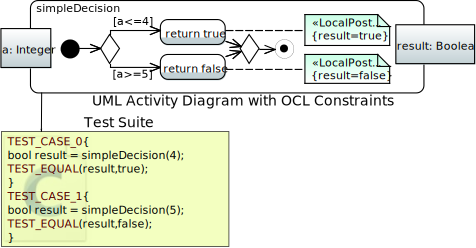
\includegraphics[width=\textwidth]{pics/IntroductoryImage.pdf}
\end{frame}

\begin{frame}
\frametitle{Outline}
\tableofcontents
\end{frame}

\section{Introduction}

\begin{frame}
\frametitle{Overview}
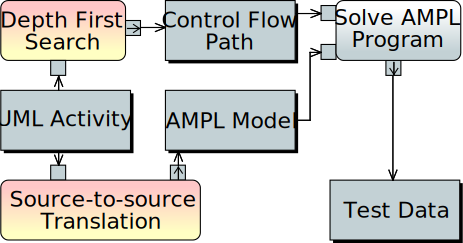
\includegraphics[width=\textwidth]{pics/SimplifiedWorkflow.pdf}
\end{frame}

\begin{frame}
\frametitle{Overview}
\begin{block}{Algorithm}
\begin{itemize}
\item Symbolic Execution
\item Constraint Solving
\item Early Infeasible Path Elimination
\item Boundary Value Analysis
\end{itemize}
\end{block}
\begin{block}{Results}
\begin{itemize}
\item Extremly high mutation scores for demo models
\item Experimental parameter tweaking
\end{itemize}
\end{block}
\end{frame}

\section{The Algorithm}
\begin{frame}
\frametitle{Outline} \tableofcontents[currentsection]
\end{frame}

\subsection{AMPL Modelling}
\begin{frame}
\frametitle{AMPL Modelling}
\begin{itemize}
  \item AMPL is a common interface to a variety of industry--strength constraint
  solvers.
  \item Source--to--source translation of UML Activity into AMPL model.
  \item Control--flow path is specified as AMPL data.
  \item Solution of an AMPL program (model + data) contains test data for a
  certain control--flow path.
\end{itemize}
\begin{block}{Supported Solvers} 
Cplex, LPSolve, Couenne, GeCoDE, ILOGCP, Minos, Gurobi, GLPK, Bonmin, Ipopt,
Xpress, \ldots
\end{block}
\begin{block}{Supported Constraint Types}
linear, non--linear, integer, mixed--integer, logical, \ldots
\end{block} 
\end{frame}

\begin{frame}[fragile]
\frametitle{Basic Example}
\begin{columns}
 \column{.39\textwidth} \ 
	\begin{block}{Activity Diagram} 
	\def\svgwidth{\textwidth}
	\scriptsize
	\import{pics/}{BasicExamples.pdf_tex}
	\end{block} 
\column{.56\textwidth} \ 
	\begin{block}{AMPL Model} 
		\begin{lstlisting}[basicstyle=\ttfamily\scriptsize,language=ampl]
param n; # Amount of executed Actions

# Variables (Property or Parameter)
var x{0..n} : integer := 1;
var y : integer := 1;

# Postconditions
set t within {0..n} default {};
s.t. t_post0{i in t} : (y)=(x[i-1]);
s.t. t_post1{i in t} : (x[i])=(x[i-1]);
set e within {0..n} default {};
s.t. e_post0{i in e} : (y)=(x[i-1]-100);
s.t. e_post0{i in e} : (x[i])=(x[i-1]);

# Guards
set d2e within {0..n} default {};
s.t. d2e_g{i in d2e} : (x[i])>=(6.0);
set d2t within {0..n} default {};
s.t. d2t_g{i in d2t} : (x[i])<=(5.0);
\end{lstlisting}
	\end{block} 
\end{columns}
\end{frame}

\subsection{Early Infeasible Path Elimination}
\begin{frame}
\frametitle{Early Infeasible Path Elimination}
	\begin{columns}[c]
		\column[c]{0.4\textwidth}
			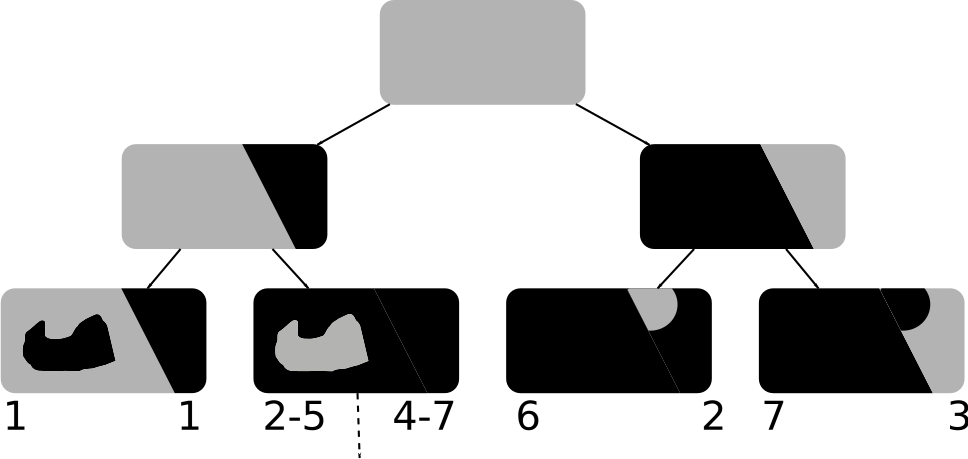
\includegraphics[width=\textwidth]{./pics/VennTree.pdf}
		\column{0.6\textwidth}
				\begin{itemize}
\item Prune control--flow paths for which no test data exist from path
search.
% \item Determine test scenarios fulfilling model structure based
% coverage criteria efficiently.
\item To ensure termination activity diagram is unrolled up to a maximum path
length.
\item If AMPL program for a sub--path is infeasible no extension of that
path can be feasible.
\item unchecked steps provide trade--of between early infeasible path
elimination and unnecessary solver invocations.
				\end{itemize}
	\end{columns}
\end{frame}

\subsection{Boundary Value Analysis}
\begin{frame}
\frametitle{Boundary Value Analysis}
\begin{columns}[c]
\column[c]{0.3\textwidth}
	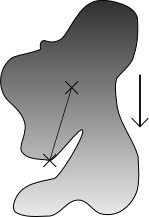
\includegraphics[width=\textwidth]{./pics/BVA.pdf}
\column{0.7\textwidth}
	\begin{itemize}
\item For a certain path constraint solvers will find any test data fulfilling
all path constraints.
\item Test data at the boundary of path constraints are most likely to trigger
an error.
\item Boundary value analysis is possible by adding a linear objective function
to the AMPL model.
	\end{itemize}
\end{columns}
\end{frame}

\section{Industrial Case Study}
\begin{frame}
\frametitle{Outline} \tableofcontents[currentsection]
\end{frame}

\begin{frame}
\frametitle{Industrial Case Study (mixed integer linear)}
\begin{itemize}
  \item The Original Model
\begin{itemize}
  \item Activity diagram consists of 21 \UMLType{Action}s, 24
  \UMLType{ControlNode}s and two nested \UMLType{LoopNode}s 
  \item C code snippets are embedded
\end{itemize}
\item Manual Adaptations
  \begin{itemize}
  \item All variables and C structs are represented by several \UMLType{Property} elements
  \item OCL constraints are deduced with an educated guess from the embedded C code snippets
  \item Hierarchical \UMLType{LoopNode}s are flattened
\end{itemize}
\end{itemize}
\begin{block}{}
The resulting constraint satisfaction problem is a mixed integer linear program
\end{block}
\end{frame}

\begin{frame}
%\frametitle{Runtime Depending on the Unchecked Steps}
\begin{tikzpicture}
\begin{axis}[
width=0.6\textwidth,
height=\textheight*0.8,
legend style={legend columns=1,at={(1.02,0.98)},anchor=north west},
xlabel={unchecked steps},
xmax=15,
ylabel={runtime $[s]$},
yticklabels={{$1$},{$10$},{$100$},{$10^3$},{$10^4$},{$10^5$}},
extra y ticks={3.6e12,2.592e14},
extra y tick labels={{1h},{3d}},
extra tick style={
        major grid style=black,
        tick align=outside,
        tick style=black
    },
minor x tick num=1,
ymajorgrids=true,
yminorgrids=true,
xmajorgrids=true,
xminorgrids=true,
ymode=log,
]
\addlegendimage{empty legend}
\addlegendentry{maximum path length}
\addplot[densely dashed, blue] table[x=PATHSEARCH_UNCHECKED_STEPS,y=time(ns)]{../Thesis/Experiment-DATA/CaseStudyUncheckedSteps90.csv};
\addlegendentry{90};
\addplot[densely dashed, green] table[x=PATHSEARCH_UNCHECKED_STEPS,y=time(ns)]{../Thesis/Experiment-DATA/CaseStudyUncheckedSteps80.csv};
\addlegendentry{80};
\addplot[densely dashed, red] table[x=PATHSEARCH_UNCHECKED_STEPS,y=time(ns);]{../Thesis/Experiment-DATA/CaseStudyUncheckedSteps70.csv};
\addlegendentry{70};
\addplot[blue] table[x=PATHSEARCH_UNCHECKED_STEPS,y=time(ns);]{../Thesis/Experiment-DATA/CaseStudyUncheckedSteps60.csv};
\addlegendentry{60};
\addplot[green] table[x=PATHSEARCH_UNCHECKED_STEPS,y=time(ns)]{../Thesis/Experiment-DATA/CaseStudyUncheckedSteps50.csv};
\addlegendentry{50};
\addplot[red] table[x=PATHSEARCH_UNCHECKED_STEPS,y={time(ns)}]{../Thesis/Experiment-DATA/CaseStudyUncheckedSteps40.csv};
\addlegendentry{40};
\end{axis}
\end{tikzpicture}
\begin{block}{}
For a maximum path length of 90, early infeasible path elimination reduces the
runtime from 3 days to less than 1 hour.
\end{block}
\end{frame}

\begin{frame}
%\frametitle{Runtime for Different Solvers}
\begin{tikzpicture}
\begin{axis}[
width=0.59\textwidth,
height=\textheight*0.8,
%legend columns=-1,
%legend to name=solvers,
legend style={at={(0.02,0.98)},anchor=north west},
xlabel={maximum path length},
ylabel={time $[s]$},
yticklabels={0,{$1$},{$10$},{$100$},{$10^3$},{$10^4$},{$10^5$}},
extra y ticks={3.6e12,2.592e14},
extra y tick labels={{1h},{3d}},
extra tick style={
        major grid style=black,
        tick align=outside,
        tick style=black
    },
minor x tick num=1,
xmin=15,
xmax=115,
ymax=1e14,
ymajorgrids=true,
yminorgrids=true,
xmajorgrids=true,
xminorgrids=true,
ymode=log,
]
\addplot[green] table[x=PATHSEARCH_MAX_PATHLENGTH,y=time(ns)] {../Thesis/Experiment-DATA/CaseStudyRuntimeCplex.csv};
\addlegendentry{Cplex};
\addplot[blue] table[x=PATHSEARCH_MAX_PATHLENGTH,y=time(ns)] {../Thesis/Experiment-DATA/CaseStudyRuntimeLPSolve.csv};
\addlegendentry{LPsolve};
\addplot[orange] table[x=PATHSEARCH_MAX_PATHLENGTH,y=time(ns)] {../Thesis/Experiment-DATA/CaseStudyRuntimeCouenne.csv};
\addlegendentry{Couenne};
\addplot[red] table[x=PATHSEARCH_MAX_PATHLENGTH,y=time(ns)] {../Thesis/Experiment-DATA/CaseStudyRuntimeGecode.csv};
\addlegendentry{GeCoDE};
\addplot[dashed] expression[no markers, domain=30:110]{2e7*1.12^(x)} node[pos=0.5,sloped,fill=white, below, opacity=1,text opacity=1] {$1.12 ^ {x}$} ;
\end{axis}
\end{tikzpicture}%
\begin{tikzpicture}
\begin{axis}[
width=0.39\textwidth,
height=\textheight*0.8,
ylabel={number of test cases},
xlabel={maximum path length},
minor x tick num=4,
ymajorgrids=true,
yminorgrids=true,
xmajorgrids=true,
xminorgrids=true,
ymode=log,
]
\addplot[blue] table[x=PATHSEARCH_MAX_PATHLENGTH,y=PathsFound]{../Thesis/Experiment-DATA/CaseStudyRuntimeLPSolve.csv};
\addplot[color=black, style=dashed] expression[no markers, domain=30:100]{1.1 ^ (x)} 
node[pos=0.5,sloped,fill=white, below, opacity=1,text opacity=1] {$1.1 ^ {x}$}
;
\end{axis}
\end{tikzpicture}
\begin{block}{}
LPsolve solved 12,849,881 mixed integer linear programming instances in 13 hours
to produce 83,000 test cases. Couenne is slower since it is optimized for mixed
integer non--linear programming
\end{block}
\end{frame}

\begin{frame}
%\frametitle{Runtime with and without Boundary Value Analysis}
\begin{tikzpicture}
\begin{axis}[
width=\textwidth,
height=0.8\textheight,
%title={Influence of boundary value analysis},
legend style={at={(0.02,0.98)},anchor=north west},
ylabel={time $[s]$},
xlabel={maximum path length},
%ytick={1e8,1e10,1e12,1e14},
yticklabels={0,{1},{10},{100},{$10^3$},{$10^4$},{$10^5$}},
extra y ticks={3.6e12,2.592e14},
extra y tick labels={{1h},{3d}},
extra tick style={
        major grid style=black,
        tick align=outside,
        tick style=black
    },
ymajorgrids=true,
yminorgrids=true,
xmajorgrids=true,
xminorgrids=true,
ymode=log,
]
\addplot[blue] table[x=PATHSEARCH_MAX_PATHLENGTH,y=time(ns)]{../Thesis/Experiment-DATA/CaseStudyRuntimeBoundaryValues.csv};
\addlegendentry{with boundary value analysis};
\addplot[red] table[x=PATHSEARCH_MAX_PATHLENGTH,y=time(ns)]{../Thesis/Experiment-DATA/CaseStudyRuntimeNoBoundaryValues.csv};
\addlegendentry{without boundary value analysis}
\end{axis}
\end{tikzpicture}%
\begin{block}{}
For a maximum path length of 70 boundary value analysis imposes extra work for
only 4.4\% of all solver invocations. This reduces to 1.1\% for a maximum path
length of 100.
\end{block}
\end{frame}

\section{Summary \& Outlook}

\begin{frame}
\frametitle{Summary}
\begin{itemize}
  \item Current constraint solvers can efficiently generate test data for
  industry scale applications.
  \item Mixed integer linear programming can be handled highly efficient.
  \item Test generation for models with mixed integer non-linear constraints is
  possible but time consuming.
  \item Early infeasible path recognition with 2 unchecked steps drastically
  reduces the runtime.
  \item Boundary value analysis can be performed with almost no effort.
  \item The ActivityTester (AcT) tool is available at
  \href{http://parteg.sourceforge.net/}{http://parteg.sourceforge.net/}.
\end{itemize}
\end{frame}

\begin{frame}
\frametitle{Outlook}
\begin{itemize}
  \item Add support for further UML/OCL modelling elements and features e.g.
  \UMLType{CallBehaviourAction} and complex data types.
  \item Reuse test goal management from ParTeG to support feasible coverage
  criteria instead of all control flow paths.
\end{itemize}
\end{frame}

\section{Demonstration \& Questions}
\begin{frame}
\begin{block}{}
\begin{center}
\Huge{Demonstration}
\end{center}
\end{block}
\end{frame}


\begin{frame}
\begin{block}{Thank you!}
\begin{center}
\Huge{Questions?}
\end{center}
\end{block}
\end{frame}

\appendix
\backupbegin
\section{Appendix}

\subsection{Meta Model}
\begin{frame}
\frametitle{The Activity Test Case Graph Model}
	\includegraphics[width=\textwidth]{../IntermediatePresentation/pics/completeMetamodelforSlideshowN.pdf}
\end{frame}

\subsection{Solvers}

\begin{frame}
\frametitle{Expressiveness and Complexity of Constraint Languages}
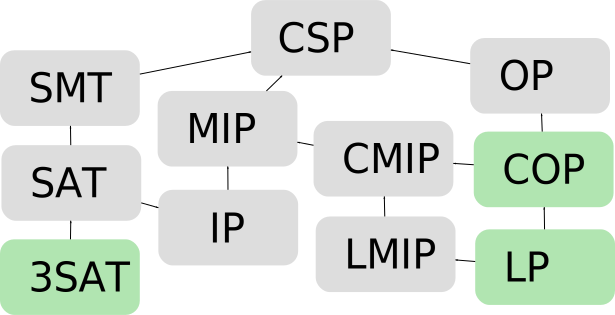
\includegraphics[width=\textwidth]{pics/ProblemLatice.pdf}
\end{frame}

\begin{frame}
\frametitle{Tested Solvers}
\begin{center}
\begin{tabular}{l r r r r r r r r}
Solver & LP & MILP & COP & OP & SAT & SMT & FCSP & MINLP\\
\hline
Cplex & \checkmark & \checkmark & & & & & &\\
IlogCP & \checkmark & \checkmark & & & \checkmark & \checkmark & \checkmark &\\
GeCoDE & & & & &\checkmark & \checkmark & \checkmark &\\
JaCoP & & & & &\checkmark & & \checkmark &\\
Couenne & \checkmark & \checkmark & \checkmark & \checkmark & & & & \checkmark\\
Gurobi & \checkmark & & \checkmark & & & & &\\
LPsolve & \checkmark &\checkmark  & & & & & &\\
Minos &\checkmark & &\checkmark & & & & &\\
% conopt & & & & & & & &\\
% knitro & & & & & & & &\\
% snopt & & & & & & & &\\
% xpress & & & & & & & &\\
% bonmin & & & & & & & &\\
% cbc & & & & & & & &\\
% ipopt & & & & & & & &\\
\hline
\end{tabular}\end{center}
\end{frame}

\subsection{Binary Counter}
\begin{frame}
\frametitle{Binary Counter}
% \def\svgwidth{\textwidth}
% \scriptsize
% \input{./pics/TriangleClasificator.pdf_tex}
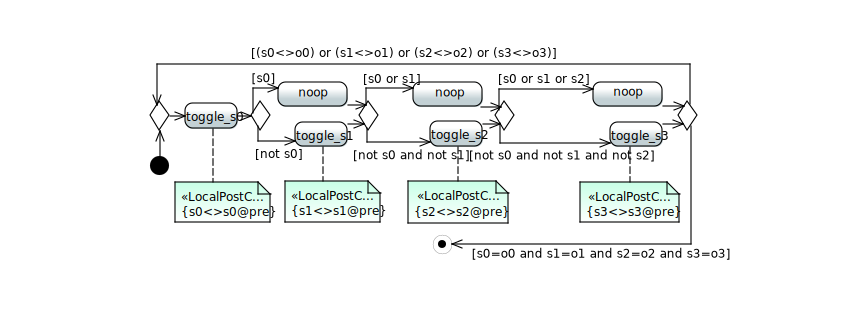
\includegraphics[width=\textwidth]{./pics/BinaryCounderSMT.pdf}
\end{frame}


\begin{frame}
\frametitle{Runtime Measurement for Different Solvers}
\begin{tikzpicture}
\begin{axis}[
width=0.598\textwidth,
height=7.5cm,
xlabel={maximum path length},
ylabel={time $[s]$},
legend style={legend columns=1,at={(0.02,0.98)},anchor=north west},
%yticklabels={0,{$1$},{$10$},{$100$},{$10^3$},{$10^4$},{$10^5$}},
extra y ticks={3.6e12,2.592e14},
extra y tick labels={{1h},{3d}},
extra tick style={
        major grid style=black,
        tick align=outside,
        tick style=black
    },
minor x tick num=1,
ymajorgrids=true,
yminorgrids=true,
xmajorgrids=true,
xminorgrids=true,
ymode=log,
xmin=5,
xmax=95,
]
\addplot[blue,no markers] table[x=PATHSEARCH_MAX_PATHLENGTH,y=time(ns)]{../Thesis/Experiment-DATA/BinaryCounterGecode+presolveSMT.csv};
\addlegendentry{GeCoDE};
\addplot[red,no markers] table[x=PATHSEARCH_MAX_PATHLENGTH,y=time(ns)]{../Thesis/Experiment-DATA/BinaryCounterJacop+presolveSMT.csv};
\addlegendentry{JaCoP};
\end{axis}
\end{tikzpicture}%
\begin{tikzpicture}
\begin{axis}[
width=0.398\textwidth,
height=7.5cm,
nodes near coords,
xmin=5,
xmax=95,
% xtick={10,20,30,40,50,60,70,80,90},
xlabel={maximum path length},
ylabel={total number of test cases},
]
\addplot+[black,mark=x,only marks] table[x=PATHSEARCH_MAX_PATHLENGTH,y=PathsFound]{../Thesis/Experiment-DATA/BinaryCounterGecode+presolveSMT.csv};
\end{axis}
\end{tikzpicture}
\end{frame}

\subsection{Case Study}
\begin{frame}
\frametitle{Runtime Depending on the Number of Test Cases}
\begin{tikzpicture}
\begin{axis}[
width=\textwidth,
height=7.5cm,
legend style={legend columns=1,at={(0.02,0.98)},anchor=north west},
xlabel={number of test cases},
ylabel={time $[s]$},
scaled y ticks = false,
% xtick scale label code/.code={\xdef\xtickscale{#1}}, 
yticklabels={0,{$1$},{$10$},{$100$},{$10^3$},{$10^4$},{$10^5$}},
extra y ticks={3.6e12,2.592e14},
extra y tick labels={{1h},{3d}},
extra tick style={
        major grid style=black,
        tick align=outside,
        tick style=black
    },
minor x tick num=1,
ymajorgrids=true,
yminorgrids=true,
xmajorgrids=true,
xminorgrids=true,
ymode=log,
xmode=log,
] 
\addplot[red] table[x=PathsFound,y=time(ns)]{../Thesis/Experiment-DATA/CaseStudyRuntimeBFS.csv};
\addlegendentry{breadth first search (Cplex)}
\addplot[green] table[x=PathsFound,y=time(ns)]{../Thesis/Experiment-DATA/CaseStudyRuntimeCplex.csv};
\addlegendentry{depth first search (Cplex)}
\addplot[blue] table[x=PathsFound,y=time(ns)]{../Thesis/Experiment-DATA/CaseStudyRuntimeLPSolve.csv};
\addlegendentry{depth first search (LPSolve)}
\addplot[color=black, style=dashed] expression[no markers, domain=1e2:1e5]{(2e7) * x}
node [pos=0.7,below,sloped,fill=white,opacity=0.85,text opacity=1] {$x^1$} 
;
\addplot[color=black, style=dashed] expression[no markers, domain=1e2:1e5]{(4e6) * x ^ (1.45)} 
node [pos=0.9,sloped,above,fill=white,opacity=0.85,text opacity=1] {$x^{1.45}$} 
;
\addplot[color=black, style=dashed] expression[no markers, domain=1e2:1e4]{(6e5) * x ^ (2)} 
node [pos=0.7,sloped,above,fill=white,opacity=0.85,text opacity=1] {$x^{2}$} 
;
\end{axis}
\end{tikzpicture}%
\end{frame}

\subsection{Algorithm}
\begin{frame}
\frametitle{Overview of the Algorithm}
\begin{block}{}
Map UML/OCL to simplified intermediate representation.
\end{block}
\begin{block}{}
Transform activity diagram into an AMPL model.
\end{block}
\begin{block}{}
Find control flow paths using depth first search with early infeasible path elimination.
\end{block}
\begin{block}{}
Solve constraint satisfaction problem for each control flow path.
\end{block}
\begin{block}{}
Output test cases as C++ unit tests using the Boost test library.
\end{block}
\end{frame}

\begin{frame}
\frametitle{Goals of Normalisation}
\begin{itemize}
  \item Ensure that the algorithm does not run into error conditions
  \item Slice relevant parts out of a huge UML model
  \item Parse embedded OCL constraints and ensure that they comply to the handled OCL subset
  \item Make implicit constraints automatically explicit
\end{itemize}
\begin{block}{}
Subsequent steps are completely independent from the UML/OCL model
\end{block}
\end{frame}

%\subsection{Abstract Test Case Generation}
\begin{frame}
\frametitle{Abstract Test Case Generation}
\begin{itemize} 
\item Determine appropriate test scenarios fulfilling model structure based coverage criteria
\item Simple breadth first or depth first search used to find control flow paths
\item Maximum path length or number of control flow paths parameter ensures termination of the algorithm
\item Infeasible paths are eliminated by solving all constraints along a path
\item How often infeasible path elimination is performed can be controlled by the parameter unchecked steps
%\item Infeasible paths elimination is performed whenever search is currently examining a real decision node and unchecked steps decision nodes have already been passed without a check
\end{itemize}
\end{frame} 


%\subsection{Specific Test Data Generation}

\begin{frame}
\frametitle{Specific Test Data Generation}
\begin{itemize} 
\item For each test scenario input data and oracle values need to be computed
\item Control flow path is symbolically executed and encoded in AMPL data
\item State--of--the--art constraint solver generates test input and the oracle value from the AMPL program
\item Boundary value analysis is possible by adding an objective function to the AMPL model
\item All generated test data is stored in a language independent unit test model
\end{itemize}
\end{frame}

%\subsection{Unit Test Synthesis}
\begin{frame}
\frametitle{Unit Test Synthesis}
\begin{itemize} 
\item Output compileable unit test code
\item Support state--of--the--art testing framework
\item Model-to-Text transformation from unit test model and activity test case graph
\item Currently C++ unit tests using the Boost test library are generated
\end{itemize}
\end{frame}

\subsection{Atego stuff}
\begin{frame}
\frametitle{Atego\textsuperscript{\textregistered} Artisan Studio Integration}
\begin{itemize}
  \item XMI format exported from Artisan Studio can be imported in Eclipse Modelling Framework.
\end{itemize}

\includegraphics[width=\textwidth]{./pics/AtegoATCGConversion.pdf}
\begin{block}{}
Better let the Normalisation directly access the Atego\textsuperscript{\textregistered} Model API.
\end{block}
\end{frame}

\subsection{Exploding Tyres}
\begin{frame}
\frametitle{Exploding Tyres (mixed integer non linear)}
% \def\svgwidth{\textwidth}
% \scriptsize
% \input{./pics/TriangleClasificator.pdf_tex}
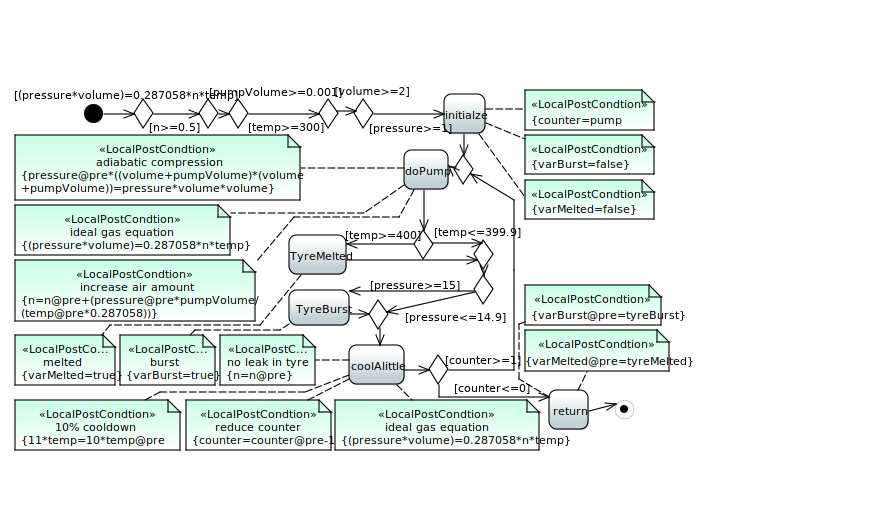
\includegraphics[width=\textwidth]{./pics/TyrePumpModel.pdf}
\end{frame}
\begin{frame}
\frametitle{Runtime with Different Solver Time Limits}
\begin{tikzpicture}
\begin{axis}[
width=0.498\textwidth,
height=7.5cm,
legend style={legend columns=1,at={(0.02,0.98)},anchor=north west},
% legend to name=myLegend,
ylabel={time $[s]$},
xlabel={maximum path length},
yticklabels={{0},{$0.1$},{$1$},{$10$},{$100$},{$10^3$},{$10^4$},{$10^5$}},
extra y ticks={3.6e12,2.592e14},
extra y tick labels={{1h},{3d}},
extra tick style={
        major grid style=black,
        tick align=outside,
        tick style=black
    },
minor x tick num=1,
ymajorgrids=true,
yminorgrids=true,
xmajorgrids=true,
xminorgrids=true,
ymode=log,
xmin=5,
xmax=75,
]
\addplot[blue,no markers] table[x=PATHSEARCH_MAX_PATHLENGTH,y=time(ns)]{../Thesis/Experiment-DATA/ExplodingTyres_10min.csv};
\addlegendentry{10min};
\addplot[red,no markers] table[x=PATHSEARCH_MAX_PATHLENGTH,y=time(ns)]{../Thesis/Experiment-DATA/ExplodingTyres_20sec.csv};
\addlegendentry{20sec};
\addplot[green,no markers] table[x=PATHSEARCH_MAX_PATHLENGTH,y=time(ns)]{../Thesis/Experiment-DATA/ExplodingTyres_5sec.csv};
\addlegendentry{5sec};
% \addplot[dash pattern=on 7pt off 3pt,no markers] table[x=PATHSEARCH_MAX_PATHLENGTH,y=time(ns)]{../Thesis/Experiment-DATA/ExplodingTyres_10s.csv};
% \addlegendentry{10sec};
% \addplot[loosely dashed,no markers] table[x=PATHSEARCH_MAX_PATHLENGTH,y=time(ns)]{../Thesis/Experiment-DATA/ExplodingTyres_60sec.csv};
% \addlegendentry{60sec};
% \addplot[solid,no markers] table[x=PATHSEARCH_MAX_PATHLENGTH,y=time(ns)]{../Thesis/Experiment-DATA/ExplodingTyres_2h.csv};
% \addlegendentry{2h};
\end{axis}
\end{tikzpicture}%
\begin{tikzpicture}
\begin{axis}[
width=0.498\textwidth,
height=7.5cm,
xlabel={maximum path length},
ylabel={number of test cases found},
minor x tick num=1,
minor y tick num=4,
ymajorgrids=true,
yminorgrids=true,
xmajorgrids=true,
xminorgrids=true,
xmin=35,
xmax=75,
]
\addplot[green,no markers] table[x=PATHSEARCH_MAX_PATHLENGTH,y=PathsFound]{../Thesis/Experiment-DATA/ExplodingTyres_5sec.csv};
%\addlegendentry{5sec};
% \addplot[dash pattern=on 7pt off 3pt,no markers] table[x=PATHSEARCH_MAX_PATHLENGTH,y=PathsFound]{Experiment-DATA/ExplodingTyres_10s.csv};
%\addlegendentry{10sec};
\addplot[red,no markers] table[x=PATHSEARCH_MAX_PATHLENGTH,y=PathsFound]{../Thesis/Experiment-DATA/ExplodingTyres_20sec.csv};
%\addlegendentry{20sec};
% \addplot[loosely dashed,no markers] table[x=PATHSEARCH_MAX_PATHLENGTH,y=PathsFound]{Experiment-DATA/ExplodingTyres_60sec.csv};
%\addlegendentry{60sec};
\addplot[blue,no markers] table[x=PATHSEARCH_MAX_PATHLENGTH,y=PathsFound]{../Thesis/Experiment-DATA/ExplodingTyres_10min.csv};
%\addlegendentry{10min};
\end{axis}
\end{tikzpicture}
\end{frame}
\begin{frame}
\frametitle{Mutation Testing the Example Model}
\begin{table}[htb]%
\begin{tabular*}{\textwidth}{@{}l@{\extracolsep{\fill}}*4r}
maximum path length     & 20      & 30      & 40        & 50\\%
\hline%
number of test cases    & 4       & 18      & 47        & 97 \\%
killed mutants          & 553     & 569     & 570       & 573 \\%
alive mutants           & 20      & 4       &  3        & 0 \\%
\hline%
mutation score          & 96.5\%  & 99.3\%  & 99.5\%    & 100\% \\%
\hline%
\end{tabular*}
\label{tab:MutationTesting}%
\end{table}
\end{frame}

\subsection{AMPL Data}
\begin{frame}[fragile]
\frametitle{AMPL Modelling}
	\begin{block}{Specify Path}
		\begin{lstlisting}[basicstyle=\ttfamily\small,language=ampl]
param l := 1;
set d2f:= 0; # guard
set f:= 1; # post condition
		\end{lstlisting}
	\end{block}
	\begin{block}{Result}
		\begin{lstlisting}[basicstyle=\ttfamily\small]
Solution determined by presolve.
a = 5
return = 0
		\end{lstlisting}
	\end{block}
\end{frame}
\backupend



\end{document}
